\documentclass[12pt]{article}
\usepackage{amsmath}
\usepackage{graphicx}
\usepackage{hyperref}
\usepackage{listings}
\usepackage{color}
\usepackage{pythonhighlight}

\title{Operating System Course Report - First Half of the Semester}
\author{B class}
\date{\today}

\begin{document}

\maketitle
\newpage

\tableofcontents
\newpage

\section{Introduction}
This report summarizes the topics covered during the first half of the Operating System course. It includes theoretical concepts, practical implementations, and assignments. The course focuses on the fundamentals of operating systems, including system architecture, process management, CPU scheduling, and deadlock handling.

\section{Course Overview}
\subsection{Objectives}
The main objectives of this course are:
\begin{itemize}
    \item To understand the basic components and architecture of a computer system.
    \item To learn process management, scheduling, and inter-process communication.
    \item To explore file systems, input/output management, and virtualization.
    \item To study the prevention and handling of deadlocks in operating systems.
\end{itemize}

\subsection{Course Structure}
The course is divided into two halves. This report focuses on the first half, which covers:
\begin{itemize}
    \item Basic Concepts and Components of Computer Systems
    \item System Performance and Metrics
    \item System Architecture of Computer Systems
    \item Process Description and Control
    \item Scheduling Algorithms
    \item Process Creation and Termination
    \item Introduction to Threads
    \item File Systems
    \item Input and Output Management
    \item Deadlock Introduction and Prevention
    \item User Interface Management
    \item Virtualization in Operating Systems
\end{itemize}

\section{Topics Covered}

\subsection{Basic Concepts and Components of Computer Systems}
This section explains the fundamental components that make up a computer system, including the CPU, memory, storage, and input/output devices.

\subsection{System Performance and Metrics}
This section introduces various system performance metrics used to measure the efficiency of a computer system, including throughput, response time, and utilization.

\subsection{System Architecture of Computer Systems}
Describes the architecture of modern computer systems, focusing on the interaction between hardware and the operating system.

\subsection{Process Description and Control}
Processes are a central concept in operating systems. This section covers:
\begin{itemize}
    \item Process states and state transitions
    \item Process control block (PCB)
    \item Context switching
\end{itemize}

\subsection{Scheduling Algorithms}
This section covers:
\begin{itemize}
    \item First-Come, First-Served (FCFS)
    \item Shortest Job Next (SJN)
    \item Round Robin (RR)
\end{itemize}
It explains how these algorithms are used to allocate CPU time to processes.

\subsection{Process Creation and Termination}
Details how processes are created and terminated by the operating system, including:
\begin{itemize}
    \item Process spawning
    \item Process termination conditions
\end{itemize}

\subsection{Introduction to Threads}
This section introduces the concept of threads and their relation to processes, covering:
\begin{itemize}
    \item Single-threaded vs. multi-threaded processes
    \item Benefits of multithreading
\end{itemize}

\begin{figure}[h]
    \centering
    \includegraphics[width=0.5\textwidth]{/Users/khawaritzmi/Unhas/os_report_mid2024/b_class/asset/example.png}  % Sesuaikan nama file dan ukurannya
    \caption{Ini adalah gambar contoh dari multithreading.}
    \label{fig:contoh_gambar}
\end{figure}

Seperti yang terlihat pada Gambar \ref{fig:contoh_gambar}, inilah cara menambahkan gambar dengan keterangan.

\subsection{File Systems}
File systems provide a way for the operating system to store, retrieve, and manage data. This section explains:
\begin{itemize}
    \item File system structure
    \item File access methods
    \item Directory management
\end{itemize}

\subsection{Input and Output Management}
Input and output management is key for handling the interaction between the system and external devices. This section includes:
\begin{itemize}
    \item Device drivers
    \item I/O scheduling
\end{itemize}

\subsection{Deadlock Introduction and Prevention}
Explores the concept of deadlocks and methods for preventing them:
\begin{itemize}
    \item Deadlock conditions
    \item Deadlock prevention techniques
\end{itemize}

\subsection{User Interface Management}
This section discusses the role of the operating system in managing the user interface. Topics covered include:
\begin{itemize}
    \item Graphical User Interface (GUI)
    \item Command-Line Interface (CLI)
    \item Interaction between the user and the operating system
\end{itemize}
\subsubsection{Command-Line Interface (CLI)}
		
		Meskipun GUI dominan dalam penggunaan umum, CLI tetap menjadi alat penting, terutama untuk \textit{administrator} sistem, pengembang, dan pengguna tingkat lanjut. CLI memungkinkan interaksi dengan sistem operasi melalui perintah teks, menawarkan tingkat kontrol dan efisiensi yang sulit dicapai melalui GUI. \cite{Shotts2019}
		
		Komponen utama CLI dalam sistem operasi modern meliputi:
		\begin{itemize}
			\item Shell: \textit{Interpreter} yang memproses perintah pengguna (contoh: Bash, Zsh, PowerShell).
			\item Terminal Emulator: Program yang menyediakan antarmuka untuk berinteraksi dengan shell.
			\item Utilitas Command-line: Kumpulan program yang dapat dijalankan dari CLI untuk berbagai tugas sistem.
			\item Scripting Capabilities: Kemampuan untuk mengotomatisasi tugas melalui skrip shell.
		\end{itemize}
		
		Keunggulan CLI meliputi:
		\begin{itemize}
			\item Efisiensi: Pengguna dapat melakukan tugas kompleks dengan cepat.
			\item Otomatisasi: Tugas berulang dapat dengan mudah diskrip dan diotomatisasi.
			\item Penggunaan Sumber Daya Rendah: CLI memerlukan sumber daya sistem yang jauh lebih sedikit dibandingkan GUI.
			\item Akses Jarak Jauh: CLI sangat cocok untuk mengelola sistem jarak jauh melalui koneksi jaringan dengan bandwidth rendah.
			\item Presisi: Memungkinkan kontrol yang sangat terperinci atas operasi sistem. \cite{Greenberg2017}
		\end{itemize}

            \begin{figure}[h]
                \centering
                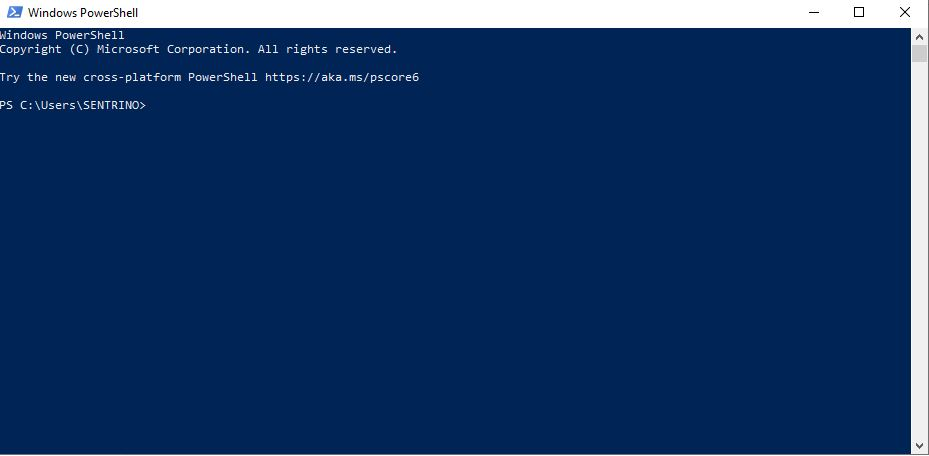
\includegraphics[width=0.6\textwidth]{asset/CLI.JPG}
                \caption{CLI IMAGE}
            \end{figure}

\subsection{Virtualization in Operating Systems}
Virtualization allows multiple operating systems to run concurrently on a single physical machine. This section explores:
\begin{itemize}
    \item Concept of virtualization
    \item Hypervisors and their types
    \item Benefits of virtualization in modern computing
\end{itemize}

\section{Assignments and Practical Work}
\subsection{Assignment 1: Process Scheduling}
Students were tasked with implementing various process scheduling algorithms (e.g., FCFS, SJN, and RR) and comparing their performance under different conditions.
\subsubsection{Kode Python dan Tabel Perbandingan Process Scheduling}
\begin{python}
    class Process:
    def __init__(self, pid, arrival_time, burst_time):
        self.pid = pid  
        self.arrival_time = arrival_time  
        self.burst_time = burst_time  
        self.completion_time = 0  
        self.turnaround_time = 0  # Turnaround time (completion - arrival)
        self.waiting_time = 0  # Waiting time (turnaround - burst)

    def calculate_times(self):
        self.turnaround_time = self.completion_time - self.arrival_time
        self.waiting_time = self.turnaround_time - self.burst_time

# First Come First Served (FCFS)
def fcfs_scheduling(processes):
    current_time = 0
    for process in sorted(processes, key=lambda p: p.arrival_time):
        if current_time < process.arrival_time:
            current_time = process.arrival_time  
        process.completion_time = current_time + process.burst_time
        process.calculate_times()
        current_time = process.completion_time

# Shortest Job Next (SJN)
def sjn_scheduling(processes):
    current_time = 0
    remaining_processes = sorted(processes, key=lambda p: (p.arrival_time, p.burst_time))

    while remaining_processes:
        # Mengambil proses dengan burst time terpendek
        available_processes = [p for p in remaining_processes if p.arrival_time <= current_time]
        if available_processes:
            next_process = min(available_processes, key=lambda p: p.burst_time)
        else:
            # jika tidak ada proses yang tiba, majukan ke arrival berikutnya
            next_process = remaining_processes[0]
            current_time = next_process.arrival_time

        current_time += next_process.burst_time
        next_process.completion_time = current_time
        next_process.calculate_times()
        remaining_processes.remove(next_process)

# Round Robin (RR) 
def rr_scheduling(processes, quantum):
    current_time = 0
    queue = sorted(processes, key=lambda p: p.arrival_time)
    time_queue = []

    while queue or time_queue:
        # tambahkan proses yang telah sampai di antrian
        while queue and queue[0].arrival_time <= current_time:
            time_queue.append(queue.pop(0))
        
        if time_queue:
            process = time_queue.pop(0)
            
            if process.burst_time > quantum:
                process.burst_time -= quantum
                current_time += quantum
                # mengembalikan proses ke antrian jika belum selesai
                time_queue.extend([p for p in queue if p.arrival_time <= current_time])
                time_queue.append(process)
            else:
                current_time += process.burst_time
                process.completion_time = current_time
                process.calculate_times()
        else:
            current_time = queue[0].arrival_time  # Maju ke arrival time selanjutnya jika antrian kosong

# Fungsi untuk mengatur ulang completion, turnaround, dan waiting times untuk proses
def reset_processes(processes):
    for process in processes:
        process.completion_time = 0
        process.turnaround_time = 0
        process.waiting_time = 0

# Contoh penggunaan:
processes = [
    Process(1, 0, 5),
    Process(2, 1, 3),
    Process(3, 2, 8),
    Process(4, 3, 6)
]

# FCFS
fcfs_scheduling(processes)
print("\n--- FCFS Scheduling ---")
print("PID\tArrival\tBurst\tCompletion\tTurnaround\tWaiting")
for process in processes:
    print(f"{process.pid}\t{process.arrival_time}\t{process.burst_time}\t"
          f"{process.completion_time}\t{process.turnaround_time}\t\t{process.waiting_time}")

# Mengatur ulang proses untuk algoritma selanjutnya
reset_processes(processes)

# SJN
sjn_scheduling(processes)
print("\n--- SJN Scheduling ---")
print("PID\tArrival\tBurst\tCompletion\tTurnaround\tWaiting")
for process in processes:
    print(f"{process.pid}\t{process.arrival_time}\t{process.burst_time}\t"
          f"{process.completion_time}\t{process.turnaround_time}\t\t{process.waiting_time}")

# Mengatur ulang proses untuk algoritma selanjutnya
reset_processes(processes)

# Round Robin Scheduling dengan Quantum = 2
quantum = 2
rr_scheduling(processes, quantum)
print("\n--- Round Robin Scheduling (Quantum = 2) ---")
print("PID\tArrival\tBurst\tCompletion\tTurnaround\tWaiting")
for process in processes:
    print(f"{process.pid}\t{process.arrival_time}\t{process.burst_time}\t"
          f"{process.completion_time}\t{process.turnaround_time}\t\t{process.waiting_time}")
\end{python}

\begin{table}[h!]
    \centering
    \resizebox{\textwidth}{!}{%
    \begin{tabular}{|c|c|c|c|c|c|c|}
    \hline
    \textbf{Algorithm} & \textbf{PID} & \textbf{Arrival Time} & \textbf{Burst Time} & \textbf{Completion Time} & \textbf{Turnaround Time} & \textbf{Waiting Time} \\ \hline
    \textbf{FCFS}      & 1            & 0                    & 5                   & 5                        & 5                        & 0                     \\ \hline
                       & 2            & 1                    & 3                   & 8                        & 7                        & 4                     \\ \hline
                       & 3            & 2                    & 8                   & 16                       & 14                       & 6                     \\ \hline
                       & 4            & 3                    & 6                   & 22                       & 19                       & 13                    \\ \hline
    \textbf{SJN}       & 1            & 0                    & 5                   & 9                        & 9                        & 4                     \\ \hline
                       & 2            & 1                    & 3                   & 4                        & 3                        & 0                     \\ \hline
                       & 3            & 2                    & 8                   & 23                       & 21                       & 13                    \\ \hline
                       & 4            & 3                    & 6                   & 15                       & 12                       & 6                     \\ \hline
    \textbf{RR}        & 1            & 0                    & 5                   & 9                        & 9                        & 4                     \\ \hline
                       & 2            & 1                    & 3                   & 6                        & 5                        & 2                     \\ \hline
                       & 3            & 2                    & 8                   & 22                       & 20                       & 12                    \\ \hline
                       & 4            & 3                    & 6                   & 18                       & 15                       & 9                     \\ \hline
    \end{tabular}%
    }
    \caption{Perbandingan FCFS, SJN, dan RR}
    \end{table}

\subsection{Assignment 2: Deadlock Handling}
In this assignment, students were asked to simulate different deadlock scenarios and explore various prevention methods.

\subsection{Assignment 3: Multithreading and Amdahl's Law}
This assignment involved designing a multithreading scenario to solve a computationally intensive problem. Students then applied **Amdahl's Law** to calculate the theoretical speedup of the program as the number of threads increased.

\subsection{Assignment 4: Simple Command-Line Interface (CLI) for User Interface Management}
Students were tasked with creating a simple **CLI** for user interface management. The CLI should support basic commands such as file manipulation (creating, listing, and deleting files), process management, and system status reporting.

\subsection{Assignment 5: File System Access}
In this assignment, students implemented file system access routines, including:
\begin{itemize}
    \item File creation and deletion
    \item Reading from and writing to files
    \item Navigating directories and managing file permissions
\end{itemize}

\section{Conclusion}
The first half of the course introduced core operating system concepts, including process management, scheduling, multithreading, and file system access. These topics provided a foundation for more advanced topics to be covered in the second half of the course.

\begin{thebibliography}{9}
    \bibitem{Shotts2019} 
                Shotts, W. (2019). \textit{The Linux command line: A complete introduction} (2nd ed.). No Starch Press.
    
    \bibitem{Greenberg2017} 
                Greenberg, J., Mates, P., \& Nam, Y. J. (2017). Robust command line interfaces: Enhancing usability while maintaining power. \textit{Journal of Systems and Software}, 133, 176-189. https://doi.org/10.1016/j.jss.2017.07.011
\end{thebibliography}

\end{document}